\section{Java Benchmarks}

In the previous assignment, we implemented several optimizations without thoroughly benchmarking them. We realized that making fundamental changes without proper performance comparison is not meaningful. The first thing we wanted to compare was using \texttt{byte} or \texttt{int} to store the attributes of a map like playerCount. At first we thought that \texttt{byte} was better because it uses less space, but then we noticed that we often had to explicitly cast to \texttt{byte} after doing some arithmetic calculations. To find out which version was better, we copied our \texttt{GameMap} class and replaced all occurrences of byte with int. In earlier tests we noticed that the order of the function calls had a significant impact on performance, so we tested the speed of the implementations in independent programs. To measure the time in Java, we used the following setup: \begin{lstlisting}
// setup, like parsing the map has already happend
long t1 = System.nanoTime();
SomeGameMapClass.checkAllPlacable();
SomeGameMapClass.getValidMove();
long t2 = System.nanoTime();
long timeIntBoolLayers = t2 - t1;
\end{lstlisting}
We recorded the results in a file and visualized them using plots, repeating each test multiple times to ensure statistically meaningful results.
\begin{figure}[H]
\centering
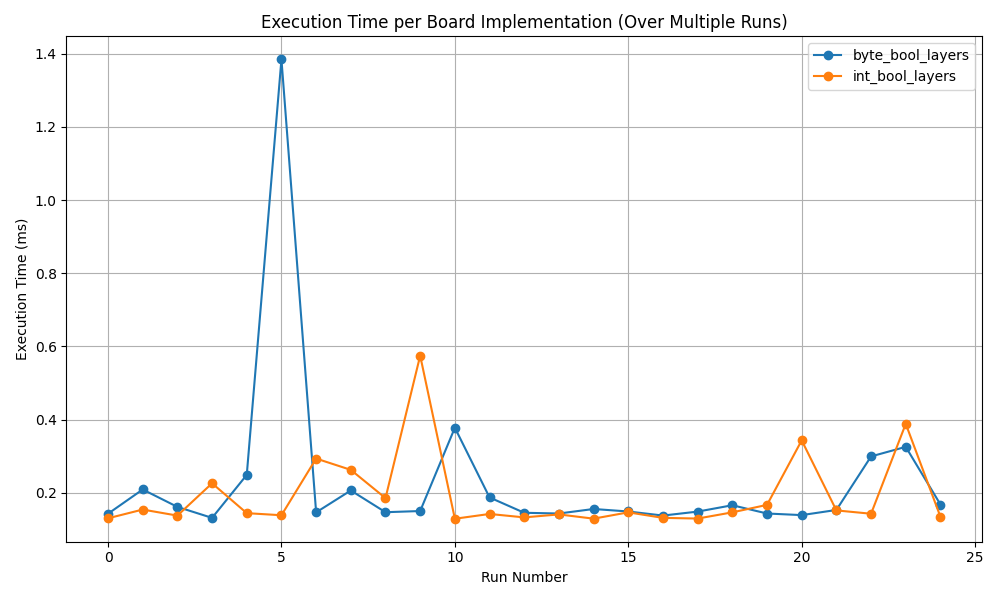
\includegraphics[width=1\linewidth]{benchmark_plots/bytevsint_original.png}
\caption{Comparison of \texttt{byte} and \texttt{int} implementations (25 iterations)}
\label{fig:25it}
\end{figure}
\begin{figure}[H]
\centering
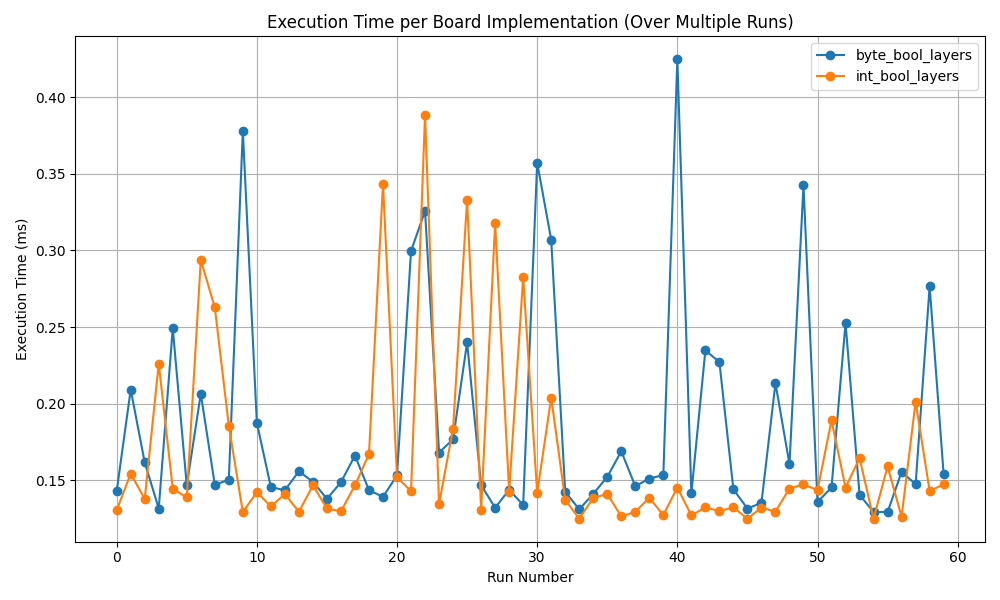
\includegraphics[width=1\linewidth]{benchmark_plots/line_longer_run.png}
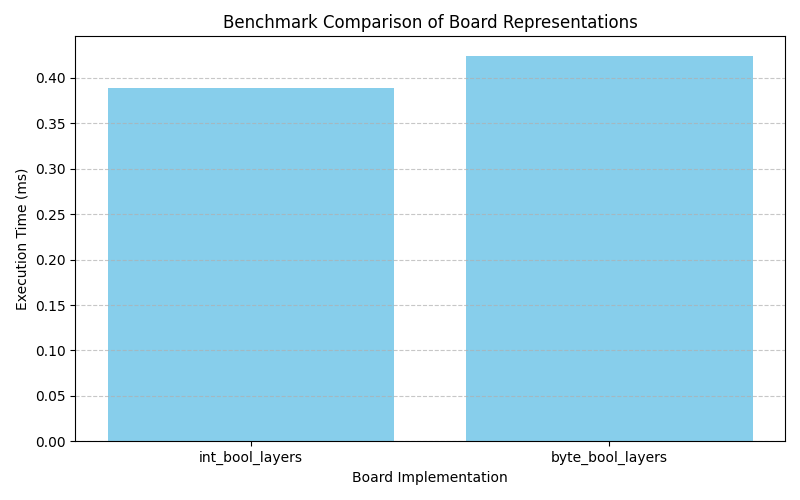
\includegraphics[width=1\linewidth]{benchmark_plots/bar_longer_run.png}
\caption{Extended comparison with 60 iterations}
\label{fig:60it}
\end{figure}
In the diagrams, the label \texttt{byte\_bool\_layers} refers to the version of the implementation that uses \texttt{byte}, \texttt{int\_bool\_layers} stands for the one that uses \texttt{int}. In the first set of tests (\autoref{fig:25it}), where each version was run 25 times, both implementations performed similarly: most executions finished in under 0.2ms. However, there were occasional spikes in execution time, making it hard to determine with implementation is faster. Those spikes might come from background activity from the JVM or some other system processes.\\[2ex]
To get a clearer picture, we ran a second round of tests with 60 iterations (\autoref{fig:60it}). This time, the results where more scattered. The increased scattering might come form external factors. We store the transitions in a hash-map, so it could also be, that a bad hash function cause some large lockup times, in some runs. \\[2ex]
Even with this variability, a trend became visible: the implementation using \texttt{int} was slightly faster on average. One likely reason is that Java automatically promotes \texttt{byte} values to \texttt{int} during arithmetic operations, and converting the results back to \texttt{byte} adds extra overhead. Besides that, using \texttt{int} also improves code readability by removing the need for repeated type casting and it becomes more clear, that we are working with numbers.\\[2ex]
Considering these points, we chose to use \texttt{int} for every number we needed to store. Although \texttt{byte} might save a small amount of memory in some scenarios, the potential gains in performance or efficiency don’t justify the added complexity.\\[2ex]
We also compared two ways of storing the map: \texttt{int[][]} and \texttt{boolean[][][]}. For a $50 \times 50$ map with the first variant we would use a \texttt{int[50][50]} array and store a number from 0 to 13 in each tile corresponding to what's on that tile. In the second case we would use an \texttt{boolean[16][50][50]} array, where we have a layer for each player and special tile. The bits set in each layer represent the occurrences of that player or special piece. We have also reserved two other layers for the valid normal moves and the valid override moves. \\[2ex]
Here we used a different approach because we wanted to increase the number of function calls to get a more rigorous result (10000 function calls). We wrote a loop, where we randomly chose which implementation we use and measured the execution time. At first we got the following graphs:
\begin{figure}[H]
\centering
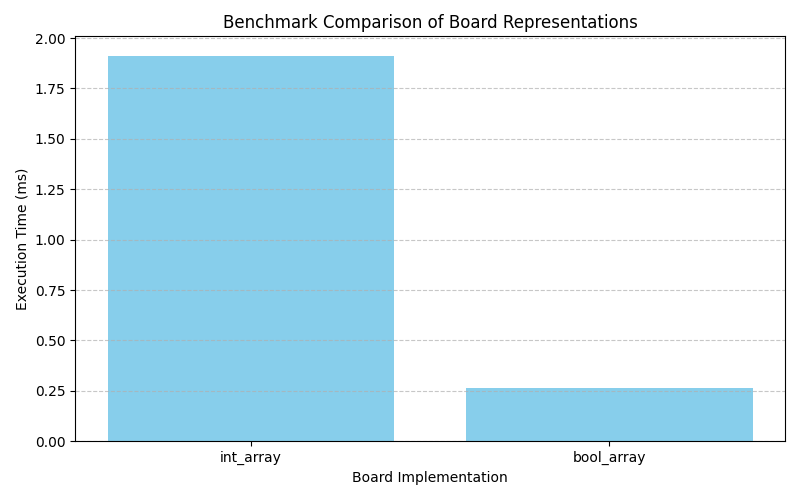
\includegraphics[width=1\linewidth]{benchmark_plots/bar_firsttry.png}
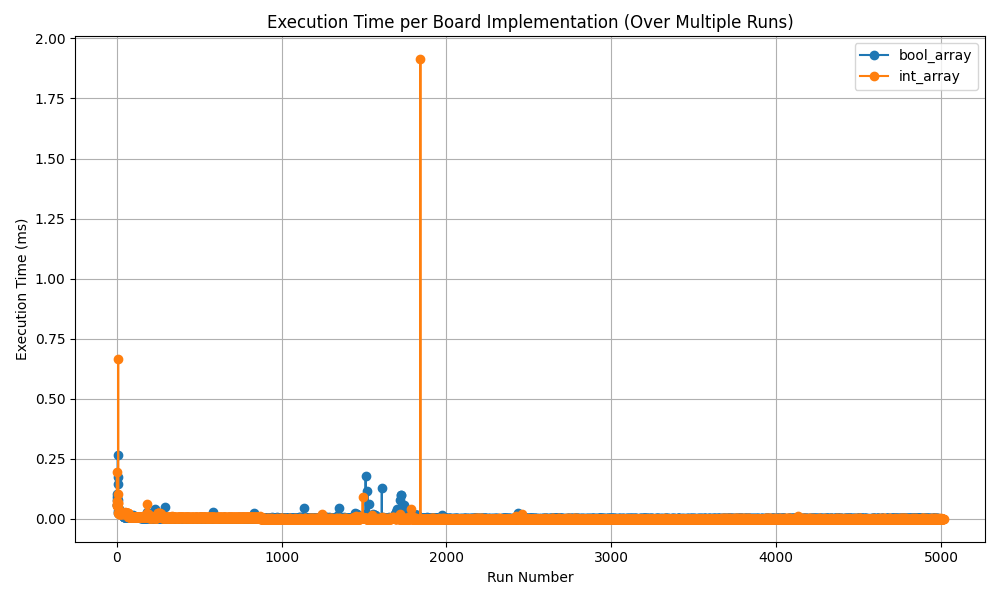
\includegraphics[width=1\linewidth]{benchmark_plots/line_firsttry.png}
\caption{First comparison, approx. 5000 iterations per Implementation}
\end{figure}

Locking at the bar diagram it seemed that using a boolean array was much faster, but analyzing the line graph, we spotted that there was a very bad run for the int array. We decided to work with averages to compensate for fluctuations. But we still wanted to calculate the averages multiple times. The following graphs where created out of data form 100 iterations, were each time an average of 100 function calls is taken:
\begin{figure}[H]
\centering
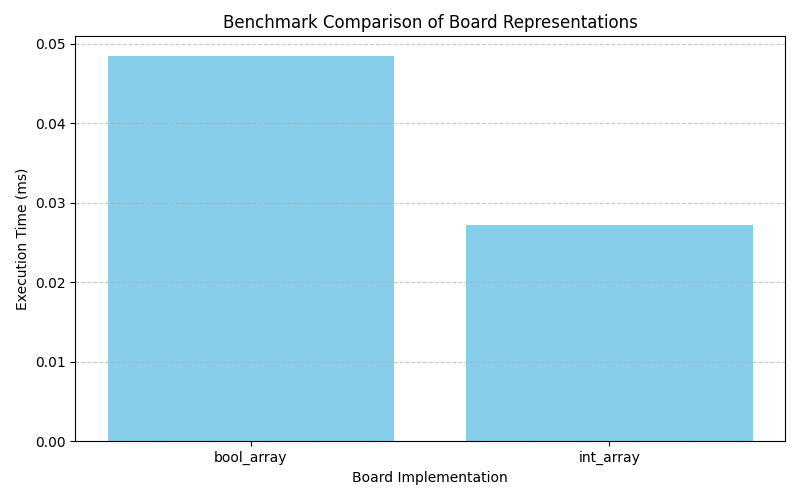
\includegraphics[width=1\linewidth]{benchmark_plots/bar_averages.png}
\caption{Comparison with averages (bar)}
\end{figure}
\begin{figure}[H]
\centering
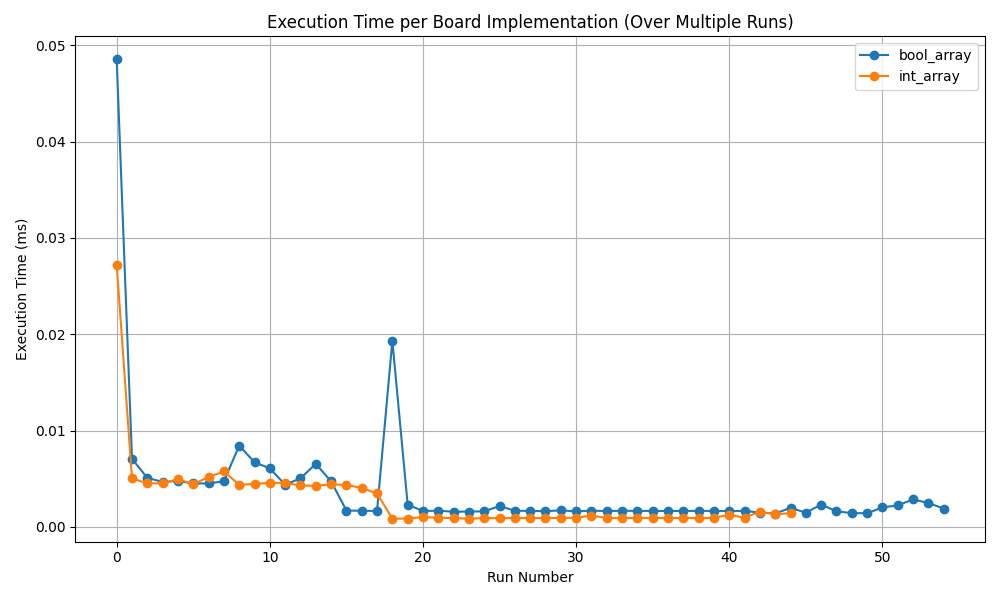
\includegraphics[width=1\linewidth]{benchmark_plots/line_averages.png}
\caption{Comparison with averages (line)}
\end{figure}
\begin{figure}[H]
\centering
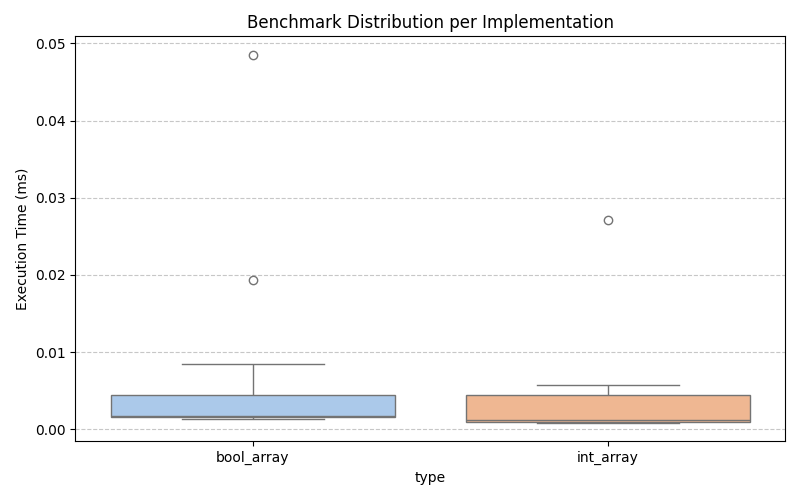
\includegraphics[width=1\linewidth]{benchmark_plots/boxplot_averages.png}
\caption{Comparison with averages (box-plot)}
\end{figure}

This time the int array performed better and the bool array had two rather bad runs. The box plots look quite similar, so it is not quite clear which version is faster.\\[2ex]
We also considered that in other maps the implementations might perform differently. So we simply ran the same code on a large map that we had downloaded from Matchpoint, this time we used 10000 iterations again, and for each iteration calculate the average of 100 function calls. The results were much clearer:
\begin{figure}[H]
\centering
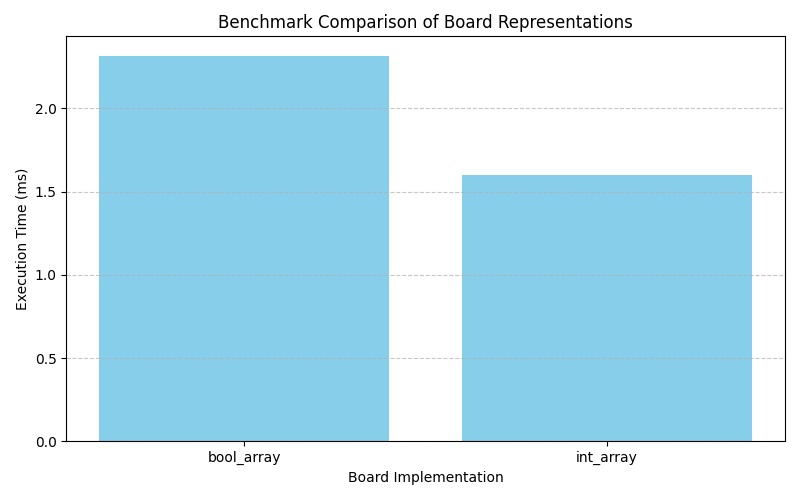
\includegraphics[width=1\linewidth]{benchmark_plots/big_map_average.png}
\caption{Comparison with averages large map  (bar)}
\end{figure}
\begin{figure}[H]
\centering
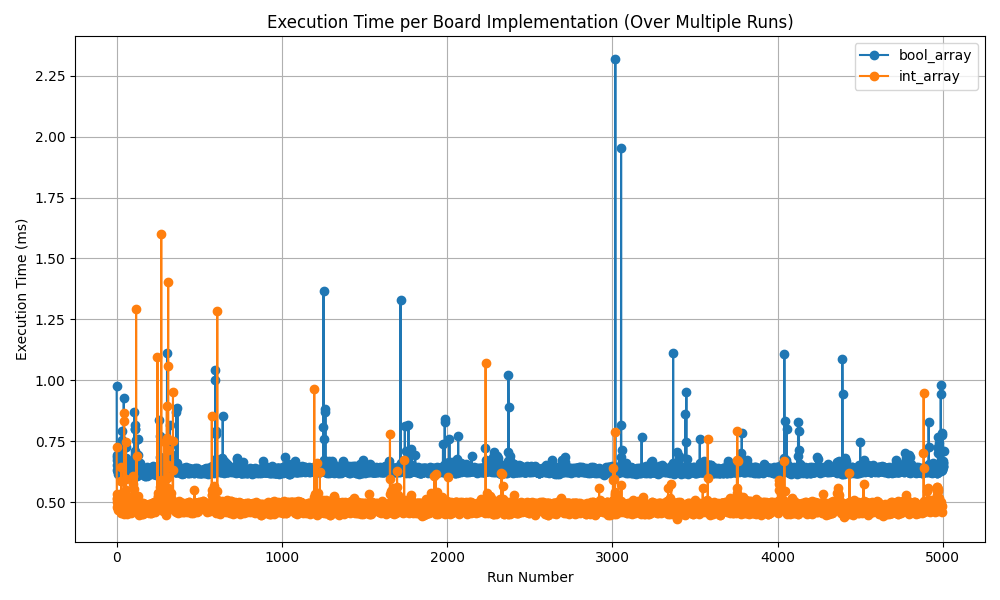
\includegraphics[width=1\linewidth]{benchmark_plots/line_big_map.png}
\caption{Comparison with averages large map (line)}
\end{figure}

All graphs show that the \texttt{int[][]} array performed better. If we look at the line we see two broad lines with a gap in between, clearly an average run with the \texttt{int[][]} array implementation was significantly faster than an average run with the \texttt{boolean[][][]} variant. To this point this was enough information to continue with the \texttt{int[][]} array.\\[2ex]
All these changes were made in Java and we found that the C++ version was still much faster. Switching to the C++ version makes the above results obsolete, but we still learned that there is absolutely no point in trying to optimise without benchmarking. In both cases, the easier to use version turned out to be the faster one.

